\documentclass{standalone}
\usepackage{tikz}
\usetikzlibrary{patterns, positioning}
\usepackage[sfdefault]{ClearSans} %% option 'sfdefault' activates Clear Sans as the default text font
\usepackage[T1]{fontenc}

\begin{document}
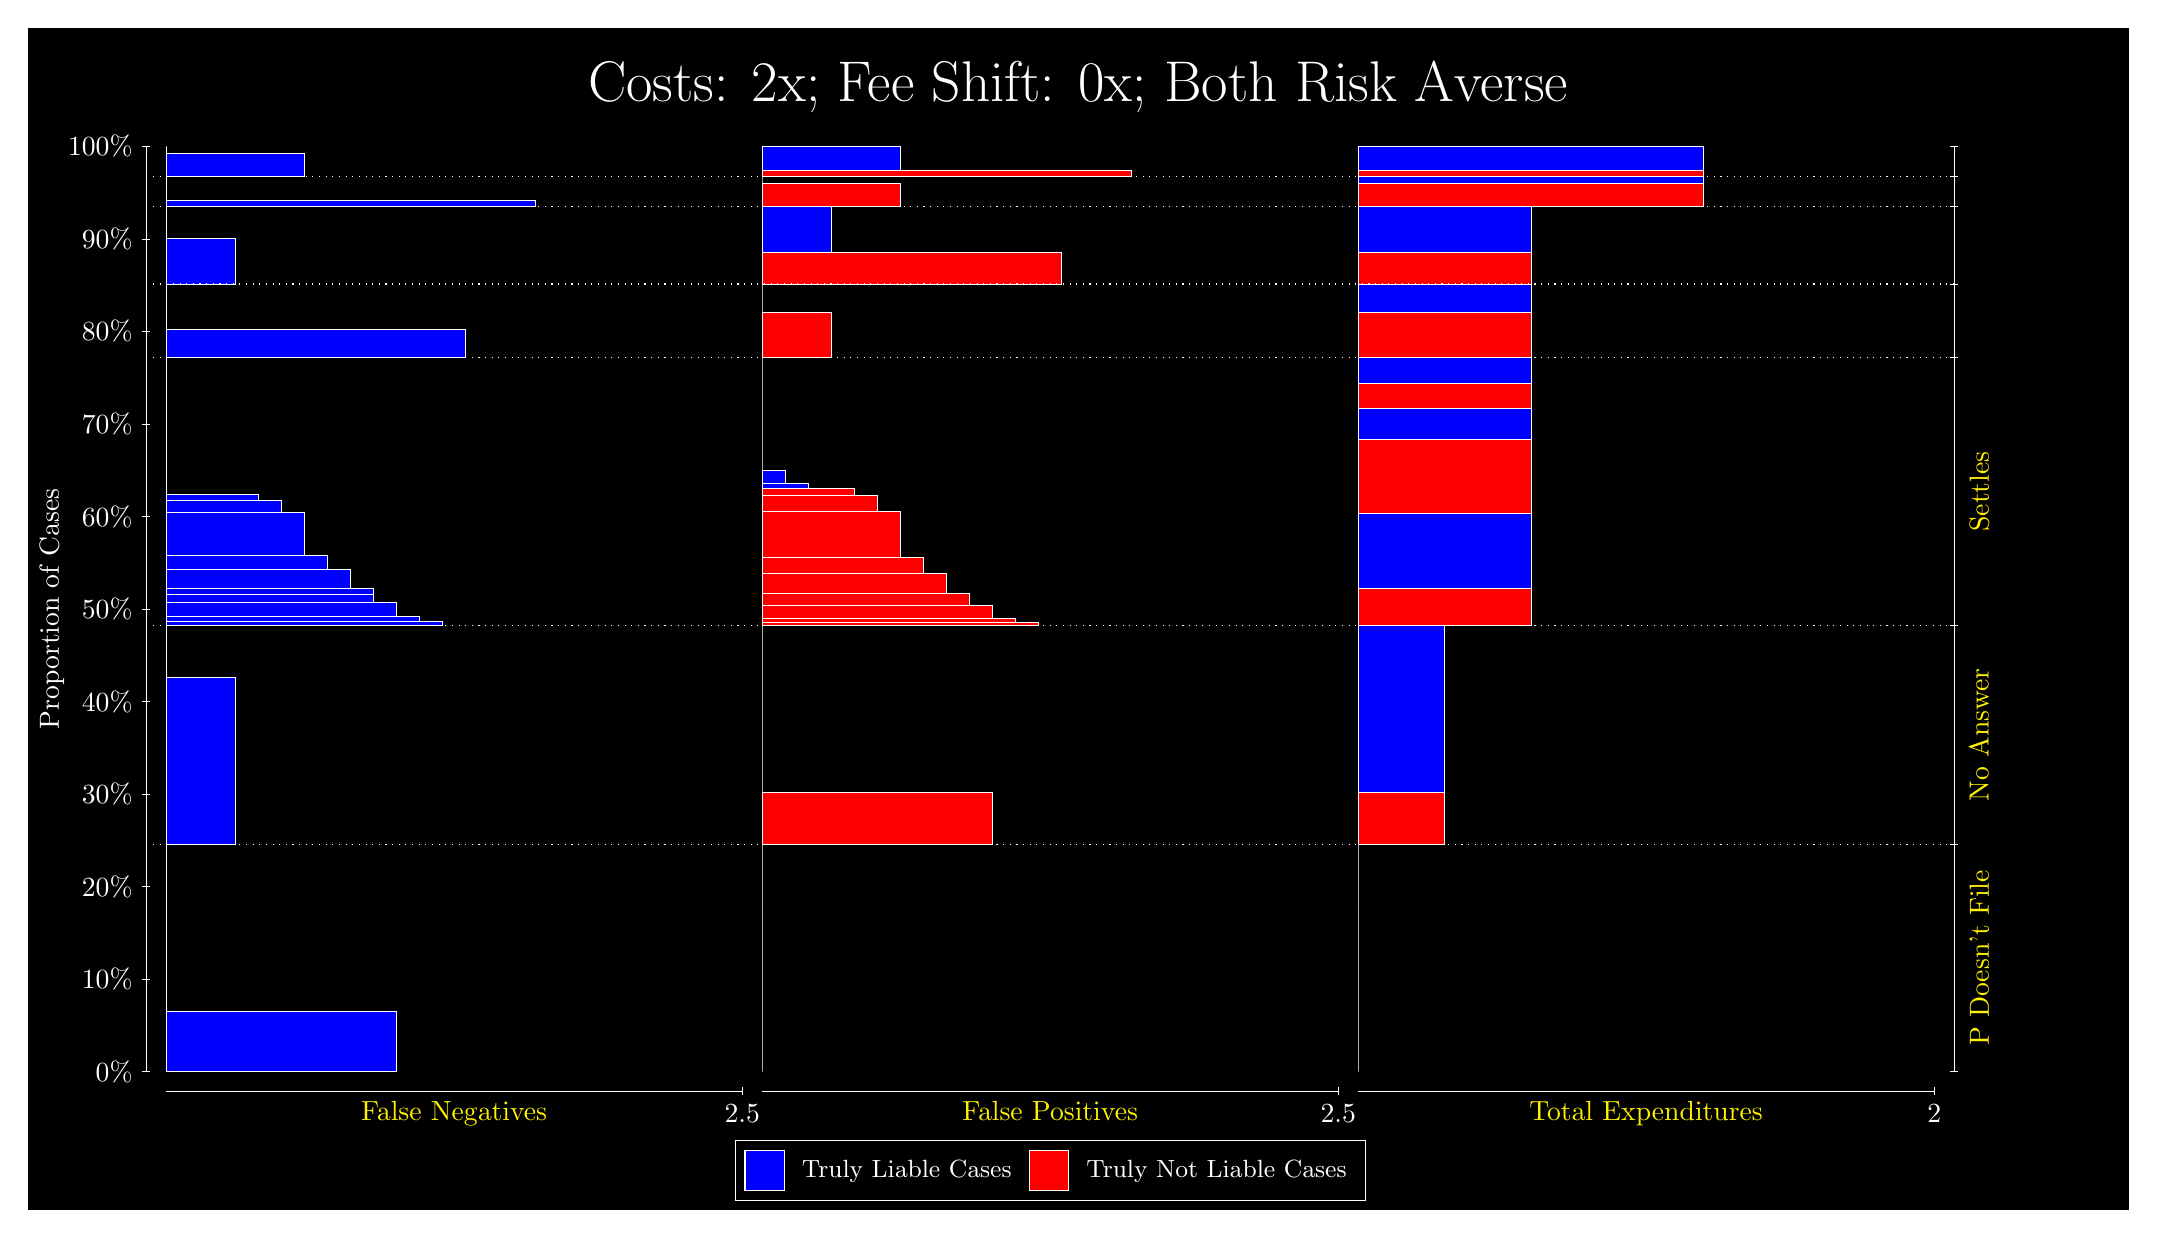
\begin{tikzpicture}
\draw[fill=black] (0,0) rectangle (26.667,15);
\draw[text=white] (0,13.5) rectangle (26.667,15) node[midway] {\huge Costs: 2x; Fee Shift: 0x; Both Risk Averse};
\draw[white, very thin] (1.5,1.75) -- (1.5,13.5);
\node[rotate=90, text=white, anchor=center] at (0.3, 7.625) {Proportion of Cases};
\draw[white, very thin] (1.45,1.75) -- (1.55,1.75);
\node[text=white, anchor=east] at (1.45, 1.75) {0\%};
\draw[white, very thin] (1.45,2.925) -- (1.55,2.925);
\node[text=white, anchor=east] at (1.45, 2.925) {10\%};
\draw[white, very thin] (1.45,4.1) -- (1.55,4.1);
\node[text=white, anchor=east] at (1.45, 4.1) {20\%};
\draw[white, very thin] (1.45,5.275) -- (1.55,5.275);
\node[text=white, anchor=east] at (1.45, 5.275) {30\%};
\draw[white, very thin] (1.45,6.45) -- (1.55,6.45);
\node[text=white, anchor=east] at (1.45, 6.45) {40\%};
\draw[white, very thin] (1.45,7.625) -- (1.55,7.625);
\node[text=white, anchor=east] at (1.45, 7.625) {50\%};
\draw[white, very thin] (1.45,8.8) -- (1.55,8.8);
\node[text=white, anchor=east] at (1.45, 8.8) {60\%};
\draw[white, very thin] (1.45,9.975) -- (1.55,9.975);
\node[text=white, anchor=east] at (1.45, 9.975) {70\%};
\draw[white, very thin] (1.45,11.15) -- (1.55,11.15);
\node[text=white, anchor=east] at (1.45, 11.15) {80\%};
\draw[white, very thin] (1.45,12.325) -- (1.55,12.325);
\node[text=white, anchor=east] at (1.45, 12.325) {90\%};
\draw[white, very thin] (1.45,13.5) -- (1.55,13.5);
\node[text=white, anchor=east] at (1.45, 13.5) {100\%};

\draw[white, very thin] (24.457,1.75) -- (24.457,13.5);
\draw[white, very thin] (24.407,1.75) -- (24.507,1.75);
\node[anchor=west] at (24.407, 1.75) {};
\draw[white, very thin] (24.407,4.6334) -- (24.507,4.6334);
\node[anchor=west] at (24.407, 4.6334) {};
\draw[white, very thin] (24.407,7.419) -- (24.507,7.419);
\node[anchor=west] at (24.407, 7.419) {};
\draw[white, very thin] (24.407,10.815) -- (24.507,10.815);
\node[anchor=west] at (24.407, 10.815) {};
\draw[white, very thin] (24.407,11.752) -- (24.507,11.752);
\node[anchor=west] at (24.407, 11.752) {};
\draw[white, very thin] (24.407,12.733) -- (24.507,12.733);
\node[anchor=west] at (24.407, 12.733) {};
\draw[white, very thin] (24.407,13.118) -- (24.507,13.118);
\node[anchor=west] at (24.407, 13.118) {};
\draw[white, very thin] (24.407,13.5) -- (24.507,13.5);
\node[anchor=west] at (24.407, 13.5) {};

\draw[white, very thin, fill=blue] (1.75,1.75) rectangle (4.6775,2.5147);
\draw[white, very thin, fill=red] (1.75,2.5147) rectangle (1.75,4.6334);
\draw[white, very thin, fill=blue] (1.75,4.6334) rectangle (2.6283,6.7561);
\draw[white, very thin, fill=red] (1.75,6.7561) rectangle (1.75,7.419);
\draw[white, very thin, fill=blue] (1.75,7.419) rectangle (5.2631,7.4624);
\draw[white, very thin, fill=blue] (1.75,7.4624) rectangle (4.9703,7.5292);
\draw[white, very thin, fill=blue] (1.75,7.5292) rectangle (4.6775,7.7078);
\draw[white, very thin, fill=blue] (1.75,7.7078) rectangle (4.3848,7.8052);
\draw[white, very thin, fill=blue] (1.75,7.8052) rectangle (4.3848,7.8815);
\draw[white, very thin, fill=blue] (1.75,7.8815) rectangle (4.092,8.1314);
\draw[white, very thin, fill=blue] (1.75,8.1314) rectangle (3.7993,8.3117);
\draw[white, very thin, fill=blue] (1.75,8.3117) rectangle (3.5065,8.8475);
\draw[white, very thin, fill=blue] (1.75,8.8475) rectangle (3.2138,9.0083);
\draw[white, very thin, fill=blue] (1.75,9.0083) rectangle (2.921,9.0786);
\draw[white, very thin, fill=red] (1.75,9.0786) rectangle (1.75,10.815);
\draw[white, very thin, fill=blue] (1.75,10.815) rectangle (5.5558,11.177);
\draw[white, very thin, fill=red] (1.75,11.177) rectangle (1.75,11.752);
\draw[white, very thin, fill=blue] (1.75,11.752) rectangle (2.6283,12.337);
\draw[white, very thin, fill=red] (1.75,12.337) rectangle (1.75,12.733);
\draw[white, very thin, fill=blue] (1.75,12.733) rectangle (6.4341,12.815);
\draw[white, very thin, fill=red] (1.75,12.815) rectangle (1.75,13.118);
\draw[white, very thin, fill=blue] (1.75,13.118) rectangle (3.5065,13.418);
\draw[white, very thin, fill=red] (1.75,13.418) rectangle (1.75,13.5);
\draw[white, very thin, fill=red] (9.3189,1.75) rectangle (9.3189,3.8687);
\draw[white, very thin, fill=blue] (9.3189,3.8687) rectangle (9.3189,4.6334);
\draw[white, very thin, fill=red] (9.3189,4.6334) rectangle (12.246,5.2963);
\draw[white, very thin, fill=blue] (9.3189,5.2963) rectangle (9.3189,7.419);
\draw[white, very thin, fill=red] (9.3189,7.419) rectangle (12.832,7.4531);
\draw[white, very thin, fill=red] (9.3189,7.4531) rectangle (12.539,7.5052);
\draw[white, very thin, fill=red] (9.3189,7.5052) rectangle (12.246,7.6678);
\draw[white, very thin, fill=red] (9.3189,7.6678) rectangle (11.954,7.8249);
\draw[white, very thin, fill=red] (9.3189,7.8249) rectangle (11.661,8.0813);
\draw[white, very thin, fill=red] (9.3189,8.0813) rectangle (11.368,8.2773);
\draw[white, very thin, fill=red] (9.3189,8.2773) rectangle (11.075,8.871);
\draw[white, very thin, fill=red] (9.3189,8.871) rectangle (10.783,9.0691);
\draw[white, very thin, fill=red] (9.3189,9.0691) rectangle (10.49,9.1555);
\draw[white, very thin, fill=blue] (9.3189,9.1555) rectangle (9.9044,9.2258);
\draw[white, very thin, fill=blue] (9.3189,9.2258) rectangle (9.6116,9.3866);
\draw[white, very thin, fill=blue] (9.3189,9.3866) rectangle (9.3189,10.815);
\draw[white, very thin, fill=red] (9.3189,10.815) rectangle (10.197,11.391);
\draw[white, very thin, fill=blue] (9.3189,11.391) rectangle (9.3189,11.752);
\draw[white, very thin, fill=red] (9.3189,11.752) rectangle (13.125,12.149);
\draw[white, very thin, fill=blue] (9.3189,12.149) rectangle (10.197,12.733);
\draw[white, very thin, fill=red] (9.3189,12.733) rectangle (11.075,13.036);
\draw[white, very thin, fill=blue] (9.3189,13.036) rectangle (9.3189,13.118);
\draw[white, very thin, fill=red] (9.3189,13.118) rectangle (14.003,13.2);
\draw[white, very thin, fill=blue] (9.3189,13.2) rectangle (11.075,13.5);
\draw[white, very thin, fill=red] (16.888,1.75) rectangle (16.888,3.8687);
\draw[white, very thin, fill=blue] (16.888,3.8687) rectangle (16.888,4.6334);
\draw[white, very thin, fill=red] (16.888,4.6334) rectangle (17.986,5.2963);
\draw[white, very thin, fill=blue] (16.888,5.2963) rectangle (17.986,7.419);
\draw[white, very thin, fill=red] (16.888,7.419) rectangle (19.083,7.8902);
\draw[white, very thin, fill=blue] (16.888,7.8902) rectangle (19.083,8.8368);
\draw[white, very thin, fill=red] (16.888,8.8368) rectangle (19.083,9.7853);
\draw[white, very thin, fill=blue] (16.888,9.7853) rectangle (19.083,10.171);
\draw[white, very thin, fill=red] (16.888,10.171) rectangle (19.083,10.488);
\draw[white, very thin, fill=blue] (16.888,10.488) rectangle (19.083,10.815);
\draw[white, very thin, fill=red] (16.888,10.815) rectangle (19.083,11.391);
\draw[white, very thin, fill=blue] (16.888,11.391) rectangle (19.083,11.752);
\draw[white, very thin, fill=red] (16.888,11.752) rectangle (19.083,12.149);
\draw[white, very thin, fill=blue] (16.888,12.149) rectangle (19.083,12.733);
\draw[white, very thin, fill=red] (16.888,12.733) rectangle (21.279,13.036);
\draw[white, very thin, fill=blue] (16.888,13.036) rectangle (21.279,13.118);
\draw[white, very thin, fill=red] (16.888,13.118) rectangle (21.279,13.2);
\draw[white, very thin, fill=blue] (16.888,13.2) rectangle (21.279,13.5);
\draw[white, dotted] (1.5,4.6334) -- (24.457,4.6334);
\draw[white, dotted] (1.5,7.419) -- (24.457,7.419);
\draw[white, dotted] (1.5,10.815) -- (24.457,10.815);
\draw[white, dotted] (1.5,11.752) -- (24.457,11.752);
\draw[white, dotted] (1.5,12.733) -- (24.457,12.733);
\draw[white, dotted] (1.5,13.118) -- (24.457,13.118);
\draw[white, very thin] (1.75,1.5) -- (9.0689,1.5);
\node[text=yellow, anchor=north] at (5.4094, 1.5) {False Negatives};
\draw[white, very thin] (9.0689,1.45) -- (9.0689,1.55);
\node[text=white, anchor=north] at (9.0689, 1.45) {2.5};

\draw[white, very thin] (9.3189,1.5) -- (16.638,1.5);
\node[text=yellow, anchor=north] at (12.978, 1.5) {False Positives};
\draw[white, very thin] (16.638,1.45) -- (16.638,1.55);
\node[text=white, anchor=north] at (16.638, 1.45) {2.5};

\draw[white, very thin] (16.888,1.5) -- (24.207,1.5);
\node[text=yellow, anchor=north] at (20.547, 1.5) {Total Expenditures};
\draw[white, very thin] (24.207,1.45) -- (24.207,1.55);
\node[text=white, anchor=north] at (24.207, 1.45) {2};

\node[text=yellow, centered, rotate=90] at (24.777, 3.1917) {P Doesn't File};
\node[text=yellow, centered, rotate=90] at (24.777, 6.0262) {No Answer};
\node[text=yellow, centered, rotate=90] at (24.777, 9.117) {Settles};





\draw (12.978300999999998,1.5) node[draw=none] (baseCoordinate) {};
\begin{scope}[align=center]
        \matrix[scale=0.5, draw=white, below=0.5cm of baseCoordinate, nodes={draw}, column sep=0.1cm]{
            \node[rectangle, draw, minimum width=0.5cm, minimum height=0.5cm, fill=blue] {}; &
            \node[draw=none, font=\small, text=white] (B) {Truly Liable Cases}; &
            \node[rectangle, draw, minimum width=0.5cm, minimum height=0.5cm, fill=red] {}; &
            \node[draw=none, font=\small, text=white] (B) {Truly Not Liable Cases}; \\
            };
\end{scope}

\end{tikzpicture}
\end{document}